\section*{Portable abstraction of hierarchical architectures for high-\/performance computing}





 \hypertarget{index_Introduction}{}\section{Introduction}\label{index_Introduction}
hwloc provides command line tools and a C API to obtain the hierarchical map of key computing elements, such as: NUMA memory nodes, shared caches, processor sockets, processor cores, processing units (logical processors or \char`\"{}threads\char`\"{}) and even I/O devices. hwloc also gathers various attributes such as cache and memory information, and is portable across a variety of different operating systems and platforms. Additionally it may assemble the topologies of multiple machines into a single one so as to let applications consult the topology of an entire fabric or cluster at once.

hwloc primarily aims at helping high-\/performance computing (HPC) applications, but is also applicable to any project seeking to exploit code and/or data locality on modern computing platforms.

Note that the hwloc project represents the merger of the libtopology project from inria and the Portable Linux Processor Affinity (PLPA) sub-\/project from Open MPI. {\itshape Both of these prior projects are now deprecated.\/} The first hwloc release was essentially a \char`\"{}re-\/branding\char`\"{} of the libtopology code base, but with both a few genuinely new features and a few PLPA-\/like features added in. Prior releases of hwloc included documentation about switching from PLPA to hwloc; this documentation has been dropped on the assumption that everyone who was using PLPA has already switched to hwloc.

hwloc supports the following operating systems:


\begin{DoxyItemize}
\item Linux (including old kernels not having sysfs topology information, with knowledge of cpusets, offline CPUs, ScaleMP vSMP, and Kerrighed support) 
\item Solaris 
\item AIX 
\item Darwin / OS X 
\item FreeBSD and its variants, such as kFreeBSD/GNU 
\item OSF/1 (a.k.a., Tru64) 
\item HP-\/UX 
\item Microsoft Windows 
\end{DoxyItemize}

Since it uses standard Operating System information, hwloc's support is mostly independant from the processor type (x86, powerpc, ...) and just relies on the Operating System support. The only exception to this is kFreeBSD, which does not support topology information, and hwloc thus uses an x86-\/only CPUID-\/based backend (which could be used for other OSes too).

To check whether hwloc works on a particular machine, just try to build it and run {\ttfamily lstopo} or {\ttfamily lstopo-\/gui}. If some things do not look right (e.g. bogus or missing cache information), see \hyperlink{index_bugs}{Questions and Bugs} below.

hwloc only reports the number of processors on unsupported operating systems; no topology information is available.

For development and debugging purposes, hwloc also offers the ability to work on \char`\"{}fake\char`\"{} topologies:


\begin{DoxyItemize}
\item Symmetrical tree of resources generated from a list of level arities 
\item Remote machine simulation through the gathering of Linux sysfs topology files 
\end{DoxyItemize}

hwloc can display the topology in a human-\/readable format, either in graphical mode (X11), or by exporting in one of several different formats, including: plain text, PDF, PNG, and FIG (see \hyperlink{index_cli_examples}{CLI Examples} below). Note that some of the export formats require additional support libraries.

hwloc offers a programming interface for manipulating topologies and objects. It also brings a powerful CPU bitmap API that is used to describe topology objects location on physical/logical processors. See the \hyperlink{index_interface}{Programming Interface} below. It may also be used to binding applications onto certain cores or memory nodes. Several utility programs are also provided to ease command-\/line manipulation of topology objects, binding of processes, and so on.

Perl bindings are available from Bernd Kallies \href{http://search.cpan.org/~bka/Sys-Hwloc-0.10/}{\tt on CPAN:}

Python bindings are available from Guy Streeter: 
\begin{DoxyItemize}
\item \href{http://people.redhat.com/streeter/}{\tt Fedora RPM and tarball}. 
\item \href{git://git.fedorahosted.org/python-hwloc.git}{\tt git tree} (\href{http://git.fedorahosted.org/git/python-hwloc.git}{\tt html}). 
\end{DoxyItemize}

 \hypertarget{index_installation}{}\section{Installation}\label{index_installation}
hwloc (\href{http://www.open-mpi.org/projects/hwloc/}{\tt http://www.open-\/mpi.org/projects/hwloc/}) is available under the BSD license. It is hosted as a sub-\/project of the overall Open MPI project (\href{http://www.open-mpi.org/}{\tt http://www.open-\/mpi.org/}). Note that hwloc does not require any functionality from Open MPI -\/-\/ it is a wholly separate (and much smaller!) project and code base. It just happens to be hosted as part of the overall Open MPI project.

Nightly development snapshots are available on the web site. Additionally, the code can be directly checked out of Subversion:


\begin{DoxyCode}
shell$ svn checkout http:\textcolor{comment}{//svn.open-mpi.org/svn/hwloc/trunk hwloc-trunk}
shell$ cd hwloc-trunk
shell$ ./autogen.sh
\end{DoxyCode}


Note that GNU Autoconf $>$=2.63, Automake $>$=1.10 and Libtool $>$=2.2.6 are required when building from a Subversion checkout.

Installation by itself is the fairly common GNU-\/based process:


\begin{DoxyCode}
shell$ ./configure --prefix=...
shell$ make
shell$ make install
\end{DoxyCode}


The hwloc command-\/line tool \char`\"{}lstopo\char`\"{} produces human-\/readable topology maps, as mentioned above. It can also export maps to the \char`\"{}fig\char`\"{} file format. Support for PDF, Postscript, and PNG exporting is provided if the \char`\"{}Cairo\char`\"{} development package can be found in \char`\"{}lstopo-\/gui\char`\"{} when hwloc is configured and build.

The hwloc core may also benefit from the following development packages: 
\begin{DoxyItemize}
\item pciutils (libpci) for I/O discovery. 
\item libnuma for memory binding and migration support on Linux. 
\item libxml2 for full XML import/export support (otherwise, the internal minimalistic parser will only be able to import XML files that were exported by the same hwloc release). See \hyperlink{a00007}{Importing and exporting topologies from/to XML files} for details. 
\end{DoxyItemize}

 \hypertarget{index_cli_examples}{}\section{CLI Examples}\label{index_cli_examples}
On a 4-\/socket 2-\/core machine with hyperthreading, the {\ttfamily lstopo-\/gui} tool may show the following graphical output:

 
\begin{DoxyImageNoCaption}
  \mbox{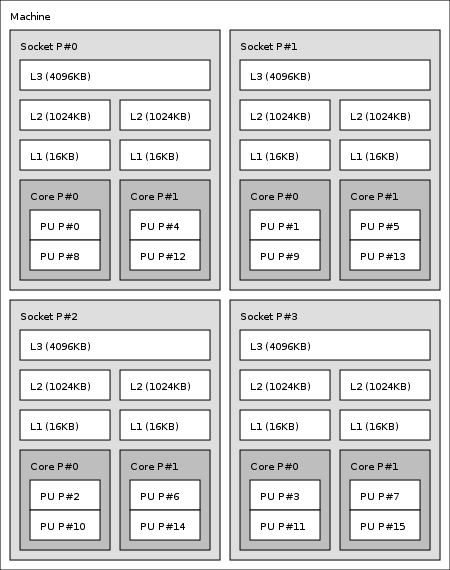
\includegraphics[width=9cm]{dudley.png}}
\end{DoxyImageNoCaption}


Here's the equivalent output in textual form:

\begin{DoxyVerb}
Machine (16GB)
  Socket L#0 + L3 L#0 (4096KB)
    L2 L#0 (1024KB) + L1 L#0 (16KB) + Core L#0
      PU L#0 (P#0)
      PU L#1 (P#8)
    L2 L#1 (1024KB) + L1 L#1 (16KB) + Core L#1
      PU L#2 (P#4)
      PU L#3 (P#12)
  Socket L#1 + L3 L#1 (4096KB)
    L2 L#2 (1024KB) + L1 L#2 (16KB) + Core L#2
      PU L#4 (P#1)
      PU L#5 (P#9)
    L2 L#3 (1024KB) + L1 L#3 (16KB) + Core L#3
      PU L#6 (P#5)
      PU L#7 (P#13)
  Socket L#2 + L3 L#2 (4096KB)
    L2 L#4 (1024KB) + L1 L#4 (16KB) + Core L#4
      PU L#8 (P#2)
      PU L#9 (P#10)
    L2 L#5 (1024KB) + L1 L#5 (16KB) + Core L#5
      PU L#10 (P#6)
      PU L#11 (P#14)
  Socket L#3 + L3 L#3 (4096KB)
    L2 L#6 (1024KB) + L1 L#6 (16KB) + Core L#6
      PU L#12 (P#3)
      PU L#13 (P#11)
    L2 L#7 (1024KB) + L1 L#7 (16KB) + Core L#7
      PU L#14 (P#7)
      PU L#15 (P#15)
\end{DoxyVerb}


Finally, here's the equivalent output in XML. Long lines were artificially broken for document clarity (in the real output, each XML tag is on a single line), and only socket \#0 is shown for brevity:

\begin{DoxyVerb}
<?xml version="1.0" encoding="UTF-8"?>
<!DOCTYPE topology SYSTEM "hwloc.dtd">
<topology>
  <object type="Machine" os_level="-1" os_index="0" cpuset="0x0000ffff" 
      complete_cpuset="0x0000ffff" online_cpuset="0x0000ffff" 
      allowed_cpuset="0x0000ffff" 
      dmi_board_vendor="Dell Computer Corporation" dmi_board_name="0RD318" 
      local_memory="16648183808">
    <page_type size="4096" count="4064498"/>
    <page_type size="2097152" count="0"/>
    <object type="Socket" os_level="-1" os_index="0" cpuset="0x00001111" 
        complete_cpuset="0x00001111" online_cpuset="0x00001111" 
        allowed_cpuset="0x00001111">
      <object type="Cache" os_level="-1" cpuset="0x00001111" 
          complete_cpuset="0x00001111" online_cpuset="0x00001111" 
          allowed_cpuset="0x00001111" cache_size="4194304" depth="3" 
          cache_linesize="64">
        <object type="Cache" os_level="-1" cpuset="0x00000101" 
            complete_cpuset="0x00000101" online_cpuset="0x00000101" 
            allowed_cpuset="0x00000101" cache_size="1048576" depth="2" 
            cache_linesize="64">
          <object type="Cache" os_level="-1" cpuset="0x00000101" 
              complete_cpuset="0x00000101" online_cpuset="0x00000101" 
              allowed_cpuset="0x00000101" cache_size="16384" depth="1" 
              cache_linesize="64">
            <object type="Core" os_level="-1" os_index="0" cpuset="0x00000101" 
                complete_cpuset="0x00000101" online_cpuset="0x00000101" 
                allowed_cpuset="0x00000101">
              <object type="PU" os_level="-1" os_index="0" cpuset="0x00000001" 
                  complete_cpuset="0x00000001" online_cpuset="0x00000001" 
                  allowed_cpuset="0x00000001"/>
              <object type="PU" os_level="-1" os_index="8" cpuset="0x00000100" 
                  complete_cpuset="0x00000100" online_cpuset="0x00000100" 
                  allowed_cpuset="0x00000100"/>
            </object>
          </object>
        </object>
        <object type="Cache" os_level="-1" cpuset="0x00001010" 
            complete_cpuset="0x00001010" online_cpuset="0x00001010" 
            allowed_cpuset="0x00001010" cache_size="1048576" depth="2" 
            cache_linesize="64">
          <object type="Cache" os_level="-1" cpuset="0x00001010" 
              complete_cpuset="0x00001010" online_cpuset="0x00001010" 
              allowed_cpuset="0x00001010" cache_size="16384" depth="1" 
              cache_linesize="64">
            <object type="Core" os_level="-1" os_index="1" cpuset="0x00001010" 
                complete_cpuset="0x00001010" online_cpuset="0x00001010" 
                allowed_cpuset="0x00001010">
              <object type="PU" os_level="-1" os_index="4" cpuset="0x00000010" 
                  complete_cpuset="0x00000010" online_cpuset="0x00000010" 
                  allowed_cpuset="0x00000010"/>
              <object type="PU" os_level="-1" os_index="12" cpuset="0x00001000" 
                  complete_cpuset="0x00001000" online_cpuset="0x00001000" 
                  allowed_cpuset="0x00001000"/>
            </object>
          </object>
        </object>
      </object>
    </object>
    <!-- ...other sockets listed here ... -->
  </object>
</topology>
\end{DoxyVerb}


On a 4-\/socket 2-\/core Opteron NUMA machine, the {\ttfamily lstopo-\/gui} tool may show the following graphical output:

 
\begin{DoxyImageNoCaption}
  \mbox{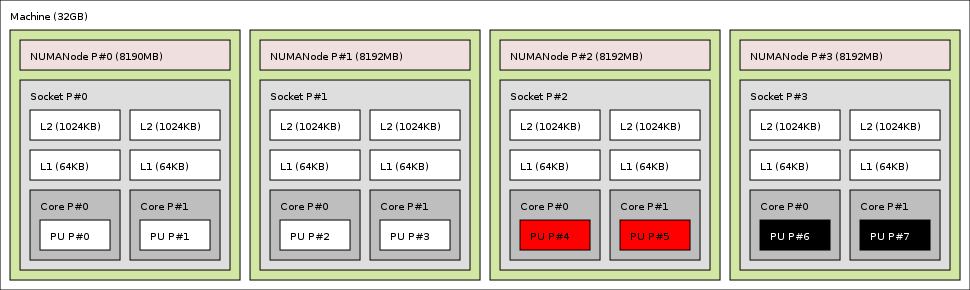
\includegraphics[width=\textwidth]{hagrid.png}}
\end{DoxyImageNoCaption}


Here's the equivalent output in textual form:

\begin{DoxyVerb}
Machine (32GB)
  NUMANode L#0 (P#0 8190MB) + Socket L#0
    L2 L#0 (1024KB) + L1 L#0 (64KB) + Core L#0 + PU L#0 (P#0)
    L2 L#1 (1024KB) + L1 L#1 (64KB) + Core L#1 + PU L#1 (P#1)
  NUMANode L#1 (P#1 8192MB) + Socket L#1
    L2 L#2 (1024KB) + L1 L#2 (64KB) + Core L#2 + PU L#2 (P#2)
    L2 L#3 (1024KB) + L1 L#3 (64KB) + Core L#3 + PU L#3 (P#3)
  NUMANode L#2 (P#2 8192MB) + Socket L#2
    L2 L#4 (1024KB) + L1 L#4 (64KB) + Core L#4 + PU L#4 (P#4)
    L2 L#5 (1024KB) + L1 L#5 (64KB) + Core L#5 + PU L#5 (P#5)
  NUMANode L#3 (P#3 8192MB) + Socket L#3
    L2 L#6 (1024KB) + L1 L#6 (64KB) + Core L#6 + PU L#6 (P#6)
    L2 L#7 (1024KB) + L1 L#7 (64KB) + Core L#7 + PU L#7 (P#7)
\end{DoxyVerb}


And here's the equivalent output in XML. Similar to above, line breaks were added and only PU \#0 is shown for brevity:

\begin{DoxyVerb}
<?xml version="1.0" encoding="UTF-8"?>
<!DOCTYPE topology SYSTEM "hwloc.dtd">
<topology>
  <object type="Machine" os_level="-1" os_index="0" cpuset="0x000000ff" 
      complete_cpuset="0x000000ff" online_cpuset="0x000000ff" 
      allowed_cpuset="0x000000ff" nodeset="0x000000ff" 
      complete_nodeset="0x000000ff" allowed_nodeset="0x000000ff" 
      dmi_board_vendor="TYAN Computer Corp" dmi_board_name="S4881 ">
    <page_type size="4096" count="0"/>
    <page_type size="2097152" count="0"/>
    <object type="NUMANode" os_level="-1" os_index="0" cpuset="0x00000003" 
        complete_cpuset="0x00000003" online_cpuset="0x00000003" 
        allowed_cpuset="0x00000003" nodeset="0x00000001" 
        complete_nodeset="0x00000001" allowed_nodeset="0x00000001" 
        local_memory="7514177536">
      <page_type size="4096" count="1834516"/>
      <page_type size="2097152" count="0"/>
      <object type="Socket" os_level="-1" os_index="0" cpuset="0x00000003" 
          complete_cpuset="0x00000003" online_cpuset="0x00000003" 
          allowed_cpuset="0x00000003" nodeset="0x00000001" 
          complete_nodeset="0x00000001" allowed_nodeset="0x00000001">
        <object type="Cache" os_level="-1" cpuset="0x00000001" 
            complete_cpuset="0x00000001" online_cpuset="0x00000001" 
            allowed_cpuset="0x00000001" nodeset="0x00000001" 
            complete_nodeset="0x00000001" allowed_nodeset="0x00000001" 
            cache_size="1048576" depth="2" cache_linesize="64">
          <object type="Cache" os_level="-1" cpuset="0x00000001" 
              complete_cpuset="0x00000001" online_cpuset="0x00000001" 
              allowed_cpuset="0x00000001" nodeset="0x00000001" 
              complete_nodeset="0x00000001" allowed_nodeset="0x00000001" 
              cache_size="65536" depth="1" cache_linesize="64">
            <object type="Core" os_level="-1" os_index="0" 
                cpuset="0x00000001" complete_cpuset="0x00000001" 
                online_cpuset="0x00000001" allowed_cpuset="0x00000001" 
                nodeset="0x00000001" complete_nodeset="0x00000001" 
                allowed_nodeset="0x00000001">
              <object type="PU" os_level="-1" os_index="0" cpuset="0x00000001" 
                  complete_cpuset="0x00000001" online_cpuset="0x00000001" 
                  allowed_cpuset="0x00000001" nodeset="0x00000001" 
                  complete_nodeset="0x00000001" allowed_nodeset="0x00000001"/>
            </object>
          </object>
        </object>
  <!-- ...more objects listed here ... -->
</topology>
\end{DoxyVerb}


On a 2-\/socket quad-\/core Xeon (pre-\/Nehalem, with 2 dual-\/core dies into each socket):

 
\begin{DoxyImageNoCaption}
  \mbox{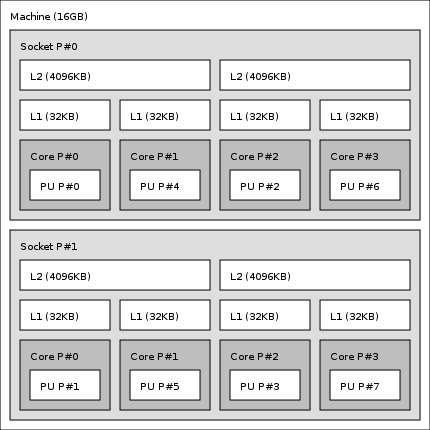
\includegraphics[width=7cm]{emmett.png}}
\end{DoxyImageNoCaption}


Here's the same output in textual form:

\begin{DoxyVerb}
Machine (16GB)
  Socket L#0
    L2 L#0 (4096KB)
      L1 L#0 (32KB) + Core L#0 + PU L#0 (P#0)
      L1 L#1 (32KB) + Core L#1 + PU L#1 (P#4)
    L2 L#1 (4096KB)
      L1 L#2 (32KB) + Core L#2 + PU L#2 (P#2)
      L1 L#3 (32KB) + Core L#3 + PU L#3 (P#6)
  Socket L#1
    L2 L#2 (4096KB)
      L1 L#4 (32KB) + Core L#4 + PU L#4 (P#1)
      L1 L#5 (32KB) + Core L#5 + PU L#5 (P#5)
    L2 L#3 (4096KB)
      L1 L#6 (32KB) + Core L#6 + PU L#6 (P#3)
      L1 L#7 (32KB) + Core L#7 + PU L#7 (P#7)
\end{DoxyVerb}


And the same output in XML (line breaks added, only PU \#0 shown):

\begin{DoxyVerb}
<?xml version="1.0" encoding="UTF-8"?>
<!DOCTYPE topology SYSTEM "hwloc.dtd">
<topology>
  <object type="Machine" os_level="-1" os_index="0" cpuset="0x000000ff" 
      complete_cpuset="0x000000ff" online_cpuset="0x000000ff" 
      allowed_cpuset="0x000000ff" dmi_board_vendor="Dell Inc." 
      dmi_board_name="0NR282" local_memory="16865292288">
    <page_type size="4096" count="4117503"/>
    <page_type size="2097152" count="0"/>
    <object type="Socket" os_level="-1" os_index="0" cpuset="0x00000055" 
        complete_cpuset="0x00000055" online_cpuset="0x00000055" 
        allowed_cpuset="0x00000055">
      <object type="Cache" os_level="-1" cpuset="0x00000011" 
          complete_cpuset="0x00000011" online_cpuset="0x00000011" 
          allowed_cpuset="0x00000011" cache_size="4194304" depth="2" 
          cache_linesize="64">
        <object type="Cache" os_level="-1" cpuset="0x00000001" 
            complete_cpuset="0x00000001" online_cpuset="0x00000001" 
            allowed_cpuset="0x00000001" cache_size="32768" depth="1" 
            cache_linesize="64">
          <object type="Core" os_level="-1" os_index="0" cpuset="0x00000001" 
              complete_cpuset="0x00000001" online_cpuset="0x00000001" 
              allowed_cpuset="0x00000001">
            <object type="PU" os_level="-1" os_index="0" cpuset="0x00000001" 
                complete_cpuset="0x00000001" online_cpuset="0x00000001" 
                allowed_cpuset="0x00000001"/>
          </object>
        </object>
        <object type="Cache" os_level="-1" cpuset="0x00000010" 
            complete_cpuset="0x00000010" online_cpuset="0x00000010" 
            allowed_cpuset="0x00000010" cache_size="32768" depth="1" 
            cache_linesize="64">
          <object type="Core" os_level="-1" os_index="1" cpuset="0x00000010" 
              complete_cpuset="0x00000010" online_cpuset="0x00000010" 
              allowed_cpuset="0x00000010">
            <object type="PU" os_level="-1" os_index="4" cpuset="0x00000010" 
                complete_cpuset="0x00000010" online_cpuset="0x00000010" 
                allowed_cpuset="0x00000010"/>
          </object>
        </object>
      </object>
  <!-- ...more objects listed here ... -->
</topology>
\end{DoxyVerb}


\hypertarget{index_interface}{}\section{Programming Interface}\label{index_interface}
The basic interface is available in \hyperlink{a00033_source}{hwloc.h}. It essentially offers low-\/level routines for advanced programmers that want to manually manipulate objects and follow links between them. Documentation for everything in \hyperlink{a00033_source}{hwloc.h} are provided later in this document. Developers should also look at \hyperlink{a00031_source}{hwloc/helper.h} (and also in this document, which provides good higher-\/level topology traversal examples).

To precisely define the vocabulary used by hwloc, a \hyperlink{a00001}{Terms and Definitions} section is available and should probably be read first.

Each hwloc object contains a cpuset describing the list of processing units that it contains. These bitmaps may be used for \hyperlink{a00049}{CPU binding} and \hyperlink{a00050}{Memory binding}. hwloc offers an extensive bitmap manipulation interface in \hyperlink{a00027_source}{hwloc/bitmap.h}.

Moreover, hwloc also comes with additional helpers for interoperability with several commonly used environments. See the \hyperlink{a00008}{Interoperability With Other Software} section for details.

The complete API documentation is available in a full set of HTML pages, man pages, and self-\/contained PDF files (formatted for both both US letter and A4 formats) in the source tarball in doc/doxygen-\/doc/.

{\bfseries NOTE:} If you are building the documentation from a Subversion checkout, you will need to have Doxygen and pdflatex installed -\/-\/ the documentation will be built during the normal \char`\"{}make\char`\"{} process. The documentation is installed during \char`\"{}make install\char`\"{} to \$prefix/share/doc/hwloc/ and your systems default man page tree (under \$prefix, of course).\hypertarget{index_portability}{}\subsection{Portability}\label{index_portability}
As shown in \hyperlink{index_cli_examples}{CLI Examples}, hwloc can obtain information on a wide variety of hardware topologies. However, some platforms and/or operating system versions will only report a subset of this information. For example, on an PPC64-\/based system with 32 cores (each with 2 hardware threads) running a default 2.6.18-\/based kernel from RHEL 5.4, hwloc is only able to glean information about NUMA nodes and processor units (PUs). No information about caches, sockets, or cores is available.

Similarly, Operating System have varying support for CPU and memory binding, e.g. while some Operating Systems provide interfaces for all kinds of CPU and memory bindings, some others provide only interfaces for a limited number of kinds of CPU and memory binding, and some do not provide any binding interface at all. Hwloc's binding functions would then simply return the ENOSYS error (Function not implemented), meaning that the underlying Operating System does not provide any interface for them. \hyperlink{a00049}{CPU binding} and \hyperlink{a00050}{Memory binding} provide more information on which hwloc binding functions should be preferred because interfaces for them are usually available on the supported Operating Systems.

Here's the graphical output from lstopo-\/gui on this platform when Simultaneous Multi-\/Threading (SMT) is enabled:

 
\begin{DoxyImageNoCaption}
  \mbox{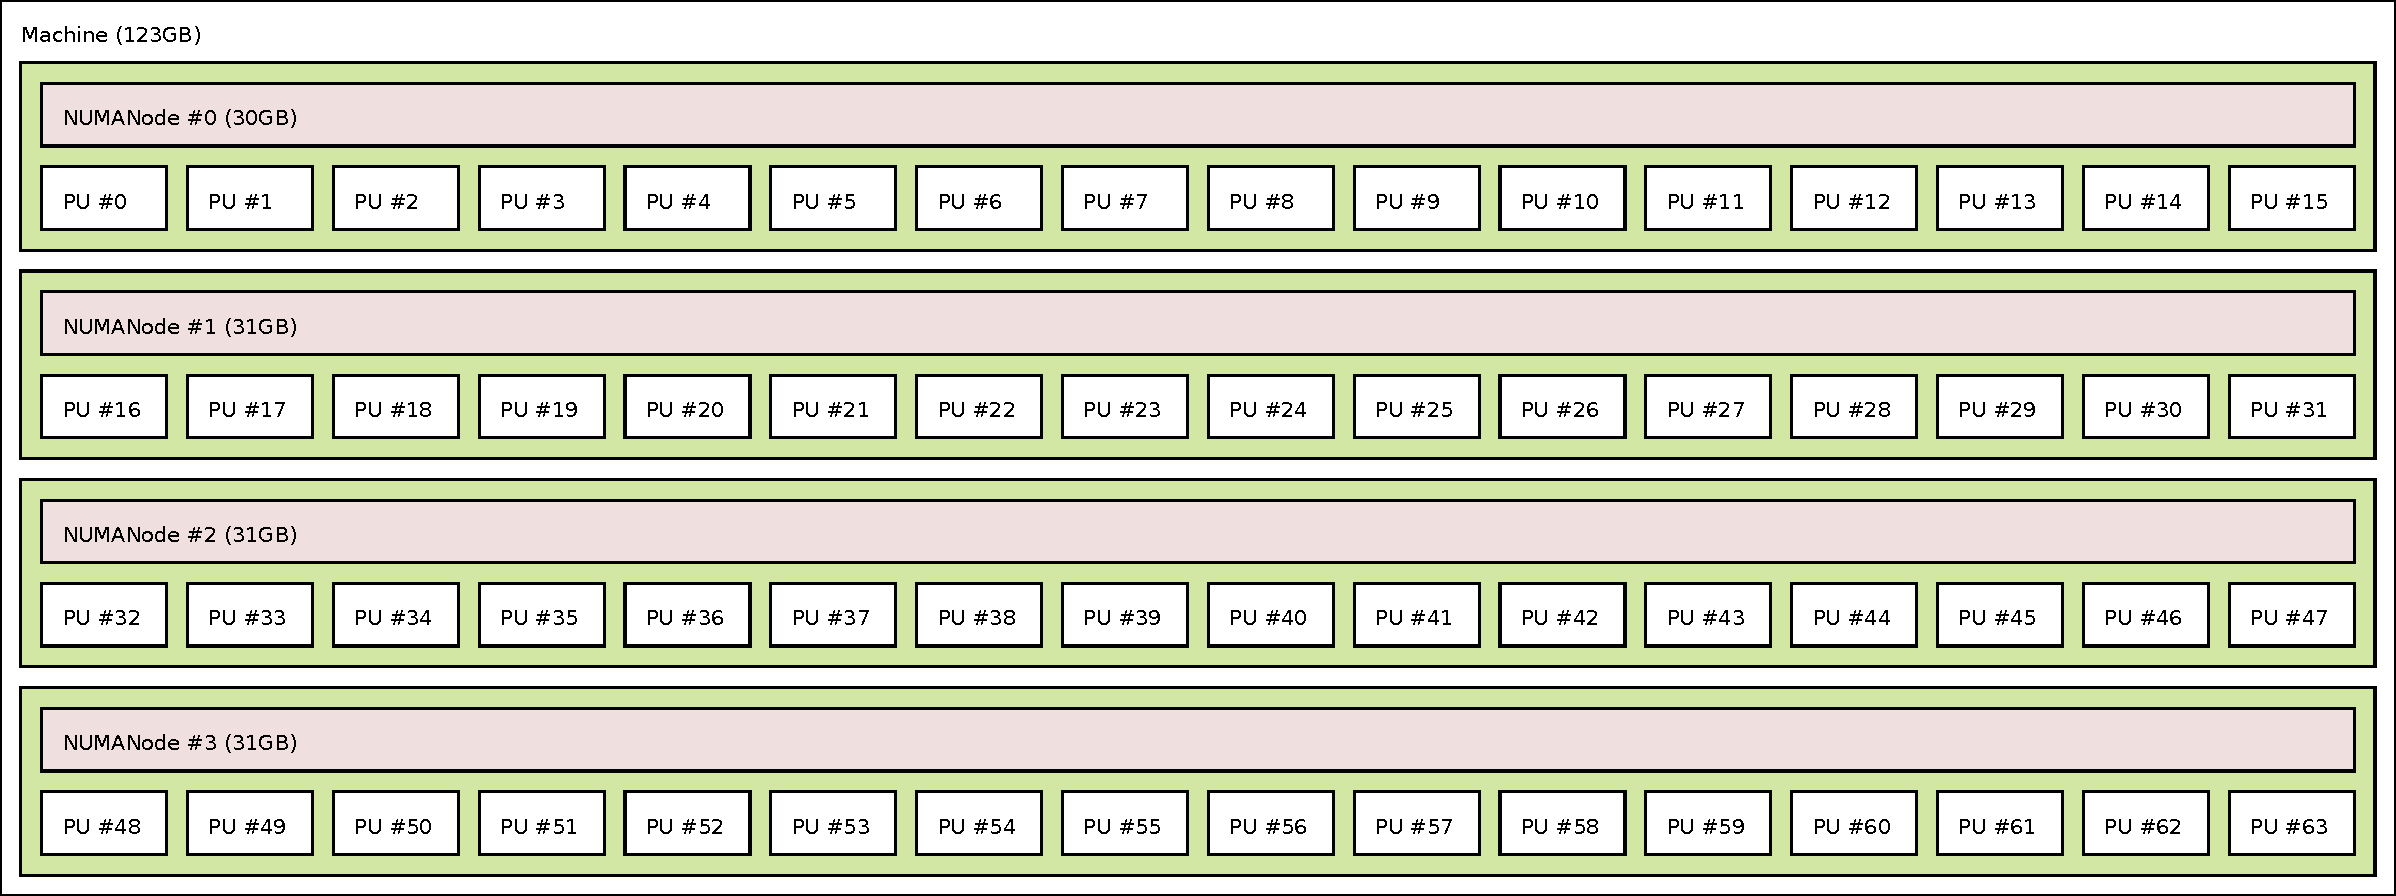
\includegraphics[width=\textwidth]{ppc64-with-smt}}
\end{DoxyImageNoCaption}


And here's the graphical output from lstopo-\/gui on this platform when SMT is disabled:

 
\begin{DoxyImageNoCaption}
  \mbox{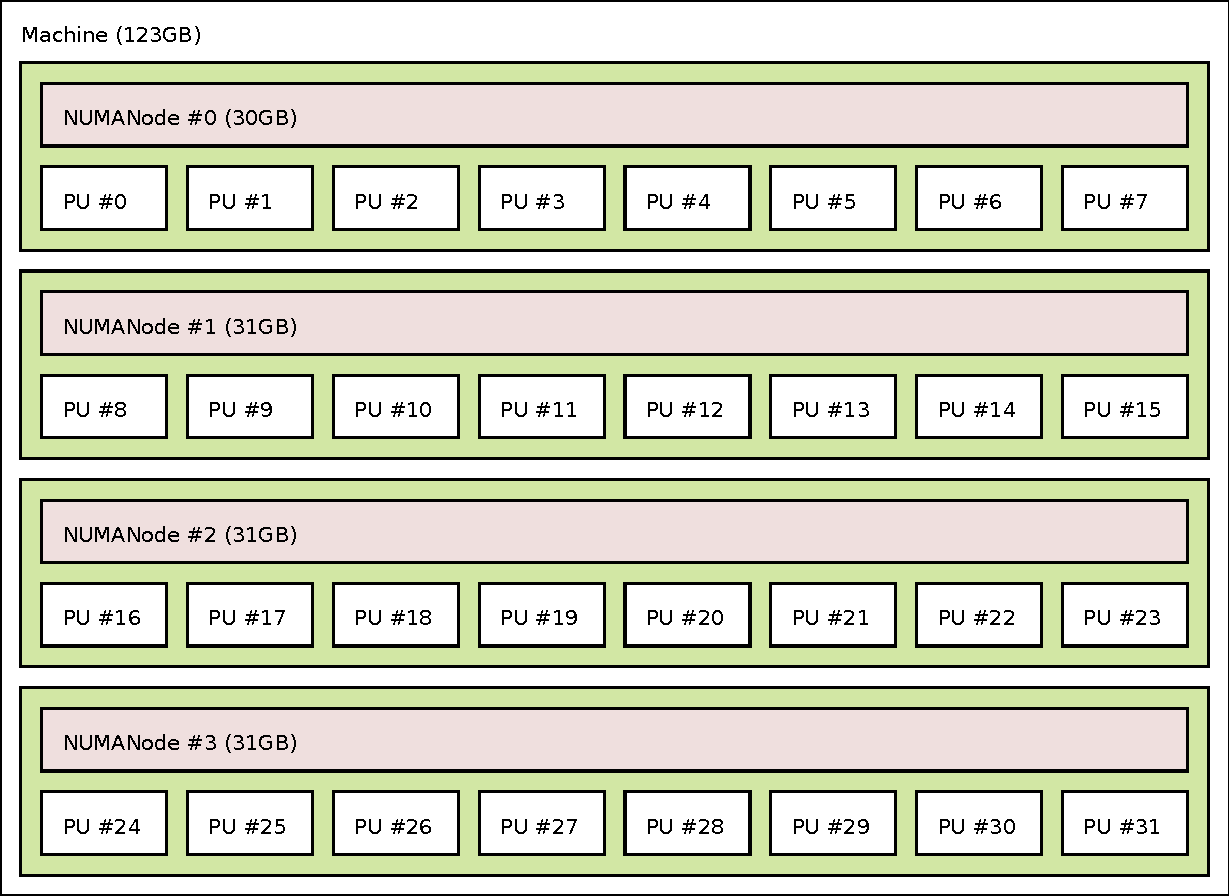
\includegraphics[width=\textwidth]{ppc64-without-smt}}
\end{DoxyImageNoCaption}


Notice that hwloc only sees half the PUs when SMT is disabled. PU \#15, for example, seems to change location from NUMA node \#0 to \#1. In reality, no PUs \char`\"{}moved\char`\"{} -\/-\/ they were simply re-\/numbered when hwloc only saw half as many. Hence, PU \#15 in the SMT-\/disabled picture probably corresponds to PU \#30 in the SMT-\/enabled picture.

This same \char`\"{}PUs have disappeared\char`\"{} effect can be seen on other platforms -\/-\/ even platforms / OSs that provide much more information than the above PPC64 system. This is an unfortunate side-\/effect of how operating systems report information to hwloc.

Note that upgrading the Linux kernel on the same PPC64 system mentioned above to 2.6.34, hwloc is able to discover all the topology information. The following picture shows the entire topology layout when SMT is enabled:

 
\begin{DoxyImageNoCaption}
  \mbox{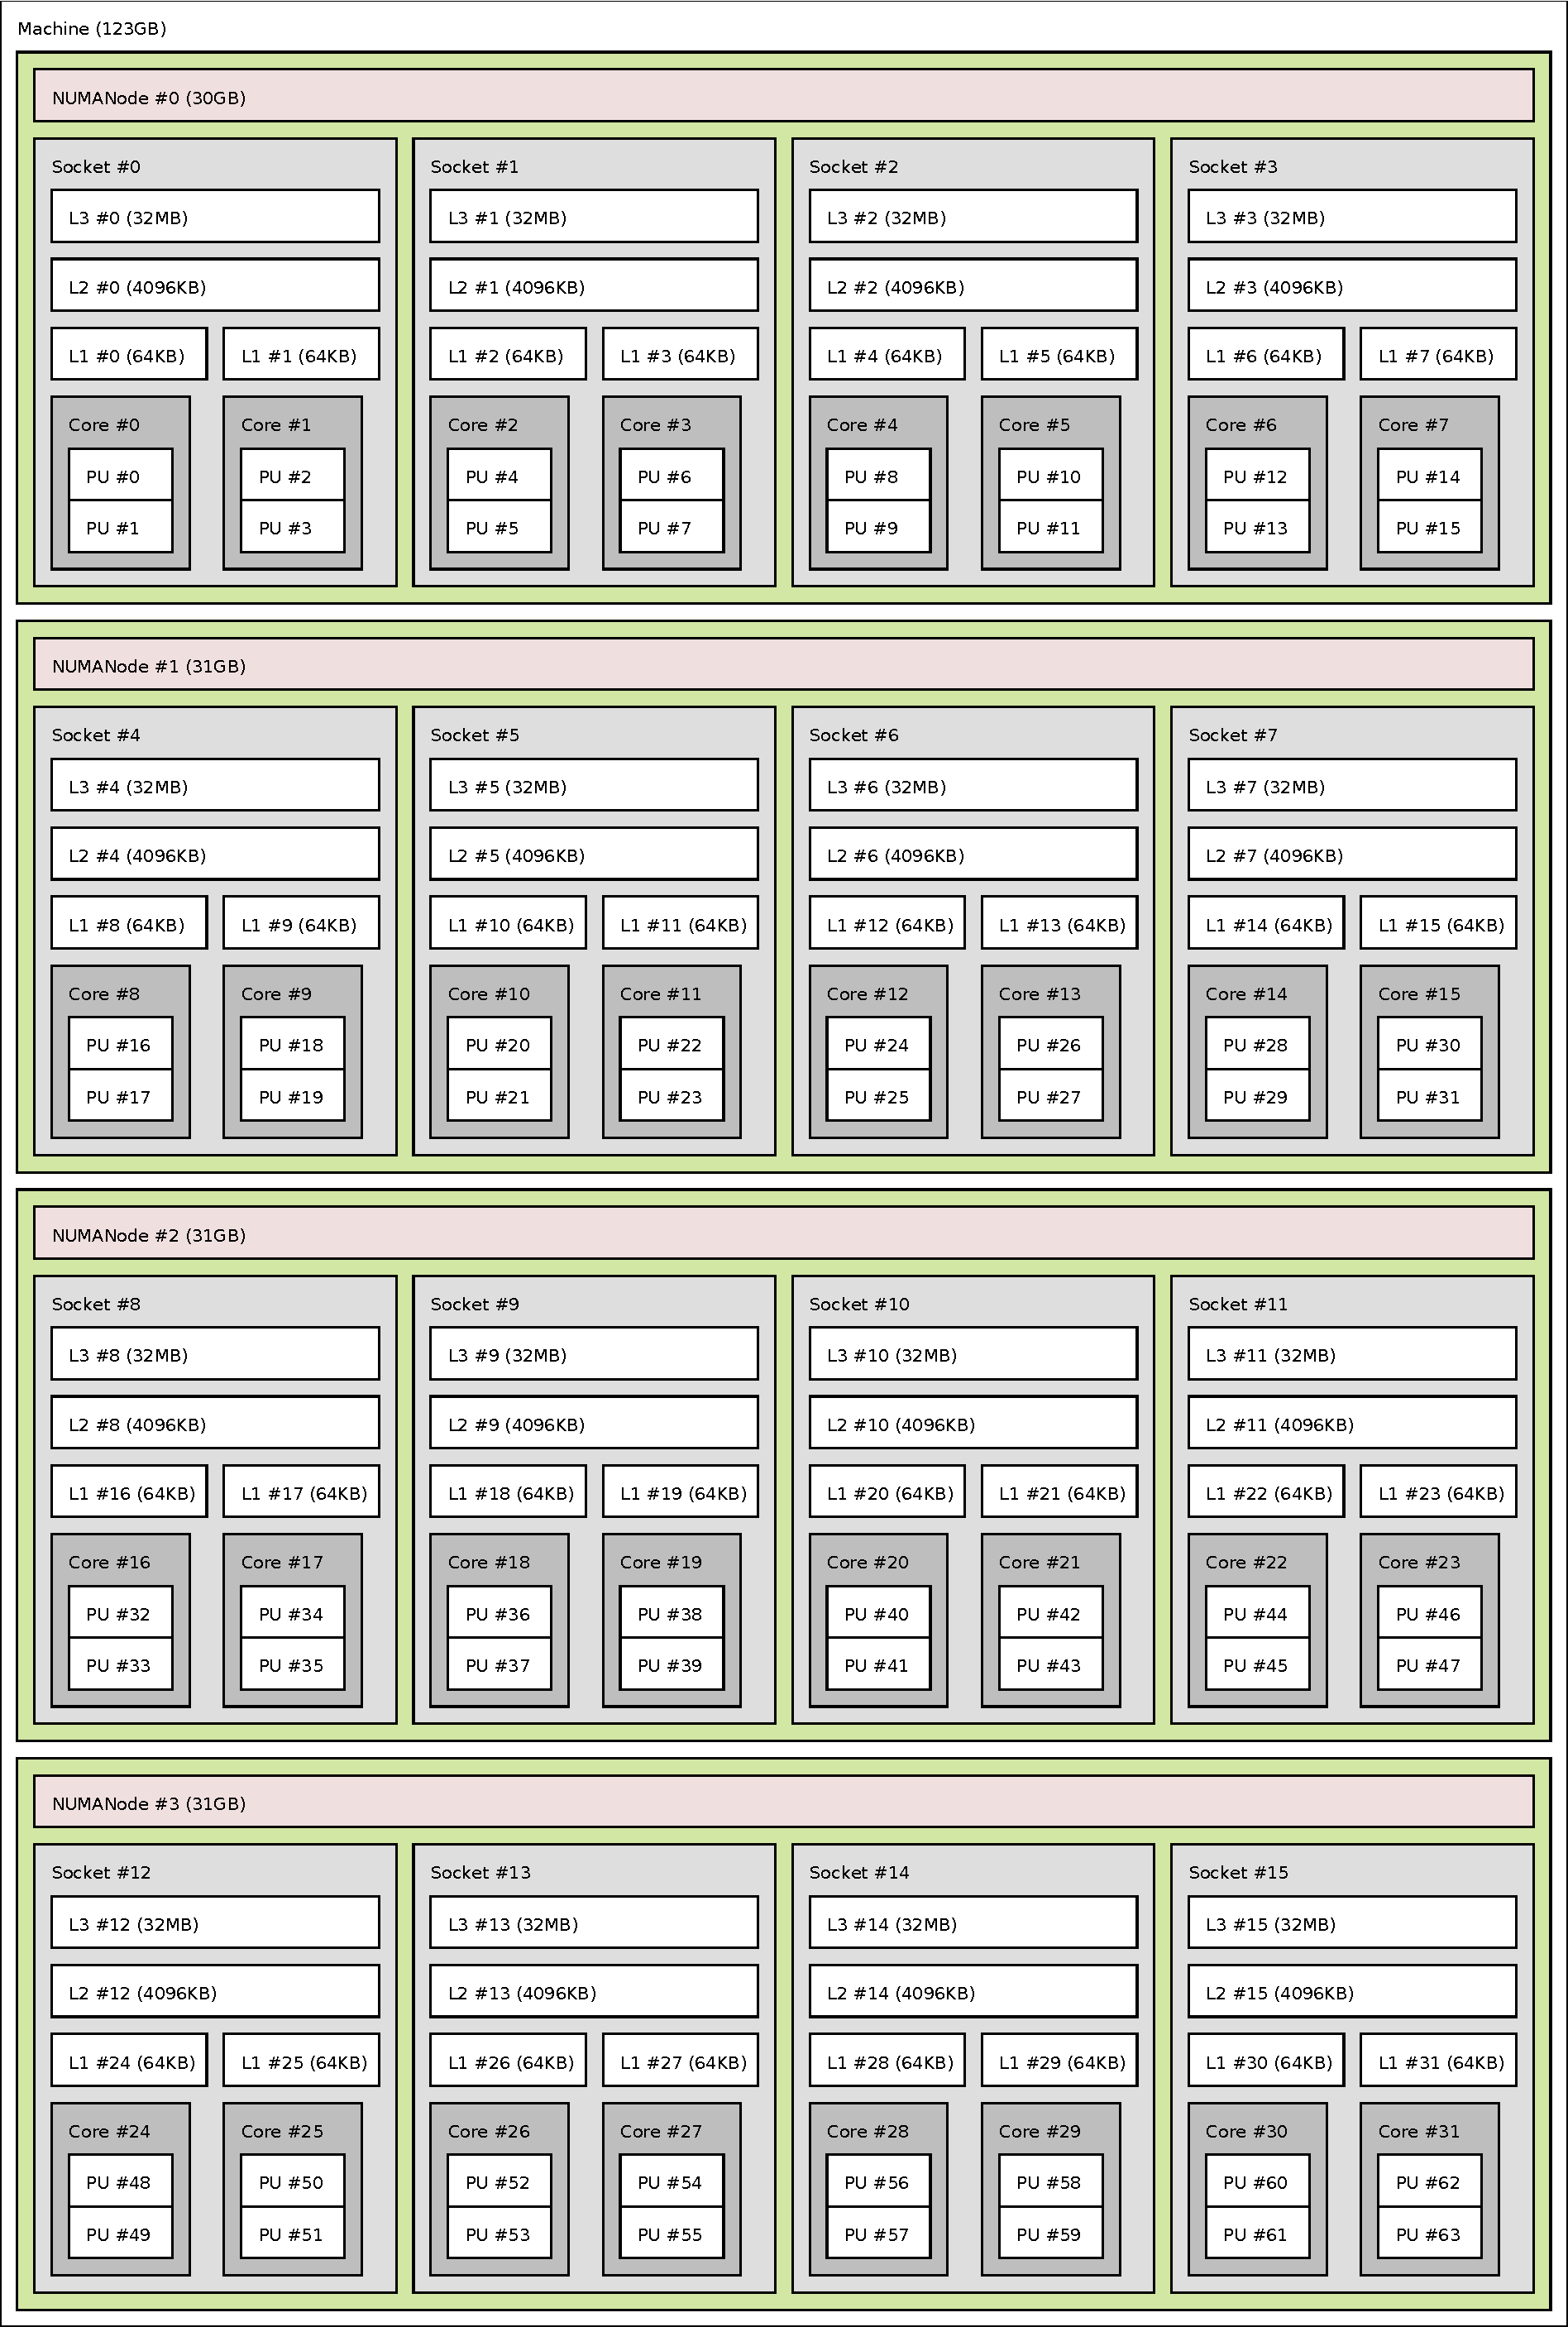
\includegraphics[width=\textwidth]{ppc64-full-with-smt}}
\end{DoxyImageNoCaption}


Developers using the hwloc API or XML output for portable applications should therefore be extremely careful to not make any assumptions about the structure of data that is returned. For example, per the above reported PPC topology, it is not safe to assume that PUs will always be descendants of cores.

Additionally, future hardware may insert new topology elements that are not available in this version of hwloc. Long-\/lived applications that are meant to span multiple different hardware platforms should also be careful about making structure assumptions. For example, there may someday be an element \char`\"{}lower\char`\"{} than a PU, or perhaps a new element may exist between a core and a PU.\hypertarget{index_interface_example}{}\subsection{API Example}\label{index_interface_example}
The following small C example (named ``hwloc-\/hello.c'') prints the topology of the machine and bring the process to the first logical processor of the second core of the machine.


\begin{DoxyCodeInclude}
\textcolor{comment}{/* Example hwloc API program.}
\textcolor{comment}{ *}
\textcolor{comment}{ * Copyright © 2009-2010 inria.  All rights reserved.}
\textcolor{comment}{ * Copyright © 2009-2011 Université Bordeaux 1}
\textcolor{comment}{ * Copyright © 2009-2010 Cisco Systems, Inc.  All rights reserved.}
\textcolor{comment}{ * See COPYING in top-level directory.}
\textcolor{comment}{ *}
\textcolor{comment}{ * hwloc-hello.c}
\textcolor{comment}{ */}

\textcolor{preprocessor}{#include <hwloc.h>}
\textcolor{preprocessor}{#include <errno.h>}
\textcolor{preprocessor}{#include <stdio.h>}
\textcolor{preprocessor}{#include <string.h>}

\textcolor{keyword}{static} \textcolor{keywordtype}{void} print\_children(\hyperlink{a00039_ga9d1e76ee15a7dee158b786c30b6a6e38}{hwloc_topology_t} topology, \hyperlink{a00016}{hwloc_obj_t} obj, 
                           \textcolor{keywordtype}{int} depth)
\{
    \textcolor{keywordtype}{char} \textcolor{keywordtype}{string}[128];
    \textcolor{keywordtype}{unsigned} i;

    \hyperlink{a00048_ga5c6a61a83f4790b421e2f62e9088446f}{hwloc_obj_snprintf}(\textcolor{keywordtype}{string}, \textcolor{keyword}{sizeof}(\textcolor{keywordtype}{string}), topology, obj, \textcolor{stringliteral}{"#"}, 0);
    printf(\textcolor{stringliteral}{"%*s%s\(\backslash\)n"}, 2*depth, \textcolor{stringliteral}{""}, \textcolor{keywordtype}{string});
    \textcolor{keywordflow}{for} (i = 0; i < obj->\hyperlink{a00016_aac3f6da35c9b57599909a44ce2b716c1}{arity}; i++) \{
        print\_children(topology, obj->\hyperlink{a00016_a04d05403da37bfe17cd63b7c7dd07b1f}{children}[i], depth + 1);
    \}
\}

\textcolor{keywordtype}{int} main(\textcolor{keywordtype}{void})
\{
    \textcolor{keywordtype}{int} depth;
    \textcolor{keywordtype}{unsigned} i, n;
    \textcolor{keywordtype}{unsigned} \textcolor{keywordtype}{long} size;
    \textcolor{keywordtype}{int} levels;
    \textcolor{keywordtype}{char} \textcolor{keywordtype}{string}[128];
    \textcolor{keywordtype}{int} topodepth;
    \hyperlink{a00039_ga9d1e76ee15a7dee158b786c30b6a6e38}{hwloc_topology_t} topology;
    \hyperlink{a00040_ga4bbf39b68b6f568fb92739e7c0ea7801}{hwloc_cpuset_t} cpuset;
    \hyperlink{a00016}{hwloc_obj_t} obj;

    \textcolor{comment}{/* Allocate and initialize topology object. */}
    \hyperlink{a00043_ga5c2d6f476af87005c7bd0811d4548b9f}{hwloc_topology_init}(&topology);

    \textcolor{comment}{/* ... Optionally, put detection configuration here to ignore}
\textcolor{comment}{       some objects types, define a synthetic topology, etc....  }
\textcolor{comment}{}
\textcolor{comment}{       The default is to detect all the objects of the machine that}
\textcolor{comment}{       the caller is allowed to access.  See Configure Topology}
\textcolor{comment}{       Detection. */}

    \textcolor{comment}{/* Perform the topology detection. */}
    \hyperlink{a00043_ga91e2e6427b95fb7339c99dbbef996e71}{hwloc_topology_load}(topology);

    \textcolor{comment}{/* Optionally, get some additional topology information}
\textcolor{comment}{       in case we need the topology depth later. */}
    topodepth = \hyperlink{a00046_ga8c30b0cec55074eb3ed34e4f2a1a9937}{hwloc_topology_get_depth}(topology);

    \textcolor{comment}{/*****************************************************************}
\textcolor{comment}{     * First example:}
\textcolor{comment}{     * Walk the topology with an array style, from level 0 (always}
\textcolor{comment}{     * the system level) to the lowest level (always the proc level).}
\textcolor{comment}{     *****************************************************************/}
    \textcolor{keywordflow}{for} (depth = 0; depth < topodepth; depth++) \{
        printf(\textcolor{stringliteral}{"*** Objects at level %d\(\backslash\)n"}, depth);
        \textcolor{keywordflow}{for} (i = 0; i < \hyperlink{a00046_ga20cfe2456f4cfdd789c9aca6d2fdd69f}{hwloc_get_nbobjs_by_depth}(topology, depth); 
             i++) \{
            \hyperlink{a00048_ga5c6a61a83f4790b421e2f62e9088446f}{hwloc_obj_snprintf}(\textcolor{keywordtype}{string}, \textcolor{keyword}{sizeof}(\textcolor{keywordtype}{string}), topology,
                       \hyperlink{a00047_gaedd78240b0c1108355586a268ec5a697}{hwloc_get_obj_by_depth}(topology, depth, i),
                       \textcolor{stringliteral}{"#"}, 0);
            printf(\textcolor{stringliteral}{"Index %u: %s\(\backslash\)n"}, i, \textcolor{keywordtype}{string});
        \}
    \}

    \textcolor{comment}{/*****************************************************************}
\textcolor{comment}{     * Second example:}
\textcolor{comment}{     * Walk the topology with a tree style.}
\textcolor{comment}{     *****************************************************************/}
    printf(\textcolor{stringliteral}{"*** Printing overall tree\(\backslash\)n"});
    print\_children(topology, \hyperlink{a00053_gadbf58f6e187efbdb3cd9a8e30311b7d7}{hwloc_get_root_obj}(topology), 0);

    \textcolor{comment}{/*****************************************************************}
\textcolor{comment}{     * Third example:}
\textcolor{comment}{     * Print the number of sockets.}
\textcolor{comment}{     *****************************************************************/}
    depth = \hyperlink{a00046_gaea7c64dd59467f5201ba87712710b14d}{hwloc_get_type_depth}(topology, \hyperlink{a00041_ggacd37bb612667dc437d66bfb175a8dc55a1ac6e07775ae4324b3fe9dbd72c785ec}{HWLOC_OBJ_SOCKET});
    \textcolor{keywordflow}{if} (depth == \hyperlink{a00046_ggaf4e663cf42bbe20756b849c6293ef575a0565ab92ab72cb0cec91e23003294aad}{HWLOC_TYPE_DEPTH_UNKNOWN}) \{
        printf(\textcolor{stringliteral}{"*** The number of sockets is unknown\(\backslash\)n"});
    \} \textcolor{keywordflow}{else} \{
        printf(\textcolor{stringliteral}{"*** %u socket(s)\(\backslash\)n"}, 
               \hyperlink{a00046_ga20cfe2456f4cfdd789c9aca6d2fdd69f}{hwloc_get_nbobjs_by_depth}(topology, depth));
    \}

    \textcolor{comment}{/*****************************************************************}
\textcolor{comment}{     * Fourth example:}
\textcolor{comment}{     * Compute the amount of cache that the first logical processor}
\textcolor{comment}{     * has above it.}
\textcolor{comment}{     *****************************************************************/}
    levels = 0;
    size = 0;
    \textcolor{keywordflow}{for} (obj = \hyperlink{a00047_ga9be4a03488cdd0fb431e4aa1cbdea895}{hwloc_get_obj_by_type}(topology, \hyperlink{a00041_ggacd37bb612667dc437d66bfb175a8dc55abca6887e80cb291353b0a0c1da83f661}{HWLOC_OBJ_PU}, 0);
         obj;
         obj = obj->\hyperlink{a00016_adc494f6aed939992be1c55cca5822900}{parent})
      \textcolor{keywordflow}{if} (obj->\hyperlink{a00016_acc4f0803f244867e68fe0036800be5de}{type} == \hyperlink{a00041_ggacd37bb612667dc437d66bfb175a8dc55a56ee0b7eca88f363b75b34fdde8c9ddc}{HWLOC_OBJ_CACHE}) \{
        levels++;
        size += obj->\hyperlink{a00016_accd40e29f71f19e88db62ea3df02adc8}{attr}->\hyperlink{a00017_ab5a8ae3bf490e6b1071fea53f7382836}{cache}.\hyperlink{a00013_abe5e788943ed04302976740c829674c0}{size};
      \}
    printf(\textcolor{stringliteral}{"*** Logical processor 0 has %d caches totaling %luKB\(\backslash\)n"}, 
           levels, size / 1024);

    \textcolor{comment}{/*****************************************************************}
\textcolor{comment}{     * Fifth example:}
\textcolor{comment}{     * Bind to only one thread of the last core of the machine.}
\textcolor{comment}{     *}
\textcolor{comment}{     * First find out where cores are, or else smaller sets of CPUs if}
\textcolor{comment}{     * the OS doesn't have the notion of a "core".}
\textcolor{comment}{     *****************************************************************/}
    depth = \hyperlink{a00052_ga081be77905201e9f42318e9974456b45}{hwloc_get_type_or_below_depth}(topology, \hyperlink{a00041_ggacd37bb612667dc437d66bfb175a8dc55ac793958f330bca371aa1535de8aff45f}{HWLOC_OBJ_CORE});

    \textcolor{comment}{/* Get last core. */}
    obj = \hyperlink{a00047_gaedd78240b0c1108355586a268ec5a697}{hwloc_get_obj_by_depth}(topology, depth,
                   \hyperlink{a00046_ga20cfe2456f4cfdd789c9aca6d2fdd69f}{hwloc_get_nbobjs_by_depth}(topology, depth) - 1);
    \textcolor{keywordflow}{if} (obj) \{
        \textcolor{comment}{/* Get a copy of its cpuset that we may modify. */}
        cpuset = \hyperlink{a00065_gaaa4ed76211cd3694dfbea2109fc440be}{hwloc_bitmap_dup}(obj->\hyperlink{a00016_a67925e0f2c47f50408fbdb9bddd0790f}{cpuset});

        \textcolor{comment}{/* Get only one logical processor (in case the core is}
\textcolor{comment}{           SMT/hyperthreaded). */}
        \hyperlink{a00065_ga4630aa1b7e08eac5b41be126194e84a1}{hwloc_bitmap_singlify}(cpuset);

        \textcolor{comment}{/* And try to bind ourself there. */}
        \textcolor{keywordflow}{if} (\hyperlink{a00049_gaf4cc194d5c0d38004a21b9f03522a7e3}{hwloc_set_cpubind}(topology, cpuset, 0)) \{
            \textcolor{keywordtype}{char} *str;
            \textcolor{keywordtype}{int} error = errno;
            \hyperlink{a00065_gad3cf87ceb58aa91656756bbb58057320}{hwloc_bitmap_asprintf}(&str, obj->\hyperlink{a00016_a67925e0f2c47f50408fbdb9bddd0790f}{cpuset});
            printf(\textcolor{stringliteral}{"Couldn't bind to cpuset %s: %s\(\backslash\)n"}, str, strerror(error));
            free(str);
        \}

        \textcolor{comment}{/* Free our cpuset copy */}
        \hyperlink{a00065_ga8e7035fe555ef96921bfb98e08519bc7}{hwloc_bitmap_free}(cpuset);
    \}

    \textcolor{comment}{/*****************************************************************}
\textcolor{comment}{     * Sixth example:}
\textcolor{comment}{     * Allocate some memory on the last NUMA node, bind some existing}
\textcolor{comment}{     * memory to the last NUMA node.}
\textcolor{comment}{     *****************************************************************/}
    \textcolor{comment}{/* Get last node. */}
    n = \hyperlink{a00046_gaba821f84ef64282d14577066e6d6547e}{hwloc_get_nbobjs_by_type}(topology, \hyperlink{a00041_ggacd37bb612667dc437d66bfb175a8dc55aaf0964881117bdedf1a5e9332cd120dd}{HWLOC_OBJ_NODE});
    \textcolor{keywordflow}{if} (n) \{
        \textcolor{keywordtype}{void} *m;
        size = 1024*1024;

        obj = \hyperlink{a00047_ga9be4a03488cdd0fb431e4aa1cbdea895}{hwloc_get_obj_by_type}(topology, \hyperlink{a00041_ggacd37bb612667dc437d66bfb175a8dc55aaf0964881117bdedf1a5e9332cd120dd}{HWLOC_OBJ_NODE}, n - 1);
        m = \hyperlink{a00050_gaeaa00714a9c4319bda0a74ca6f8720e8}{hwloc_alloc_membind_nodeset}(topology, size, obj->\hyperlink{a00016_a08f0d0e16c619a6e653526cbee4ffea3}{nodeset},
                \hyperlink{a00050_ggac9764f79505775d06407b40f5e4661e8a18675bb80ebc1bce5b652e9de8f3998c}{HWLOC_MEMBIND_DEFAULT}, 0);
        \hyperlink{a00050_ga986d9b4cc76da592c4b937c6cb7d9d56}{hwloc_free}(topology, m, size);

        m = malloc(size);
        \hyperlink{a00050_gade5e2c28ea8475a479bf2b1df36c6ccd}{hwloc_set_area_membind_nodeset}(topology, m, size, obj->\hyperlink{a00016_a08f0d0e16c619a6e653526cbee4ffea3}{nodeset},
                \hyperlink{a00050_ggac9764f79505775d06407b40f5e4661e8a18675bb80ebc1bce5b652e9de8f3998c}{HWLOC_MEMBIND_DEFAULT}, 0);
        free(m);
    \}

    \textcolor{comment}{/* Destroy topology object. */}
    \hyperlink{a00043_ga6040925d3ee4bbb2647f2a321aca5f4b}{hwloc_topology_destroy}(topology);

    \textcolor{keywordflow}{return} 0;
\}
\end{DoxyCodeInclude}


hwloc provides a {\ttfamily pkg-\/config} executable to obtain relevant compiler and linker flags. For example, it can be used thusly to compile applications that utilize the hwloc library (assuming GNU Make):

\begin{DoxyVerb}
CFLAGS += $(pkg-config --cflags hwloc)
LDLIBS += $(pkg-config --libs hwloc)
cc hwloc-hello.c $(CFLAGS) -o hwloc-hello $(LDLIBS)
\end{DoxyVerb}


On a machine with 4GB of RAM and 2 processor sockets -\/-\/ each socket of which has two processing cores -\/-\/ the output from running {\ttfamily hwloc-\/hello} could be something like the following:

\begin{DoxyVerb}
shell$ ./hwloc-hello
*** Objects at level 0
Index 0: Machine(3938MB)
*** Objects at level 1
Index 0: Socket#0
Index 1: Socket#1
*** Objects at level 2
Index 0: Core#0
Index 1: Core#1
Index 2: Core#3
Index 3: Core#2
*** Objects at level 3
Index 0: PU#0
Index 1: PU#1
Index 2: PU#2
Index 3: PU#3
*** Printing overall tree
Machine(3938MB)
  Socket#0
    Core#0
      PU#0
    Core#1
      PU#1
  Socket#1
    Core#3
      PU#2
    Core#2
      PU#3
*** 2 socket(s)
shell$ 
\end{DoxyVerb}


 \hypertarget{index_bugs}{}\section{Questions and Bugs}\label{index_bugs}
Questions should be sent to the devel mailing list (\href{http://www.open-mpi.org/community/lists/hwloc.php}{\tt http://www.open-\/mpi.org/community/lists/hwloc.php}). Bug reports should be reported in the tracker (\href{https://svn.open-mpi.org/trac/hwloc/}{\tt https://svn.open-\/mpi.org/trac/hwloc/}).

If hwloc discovers an incorrect topology for your machine, the very first thing you should check is to ensure that you have the most recent updates installed for your operating system. Indeed, most of hwloc topology discovery relies on hardware information retrieved through the operation system (e.g., via the /sys virtual filesystem of the Linux kernel). If upgrading your OS or Linux kernel does not solve your problem, you may also want to ensure that you are running the most recent version of the BIOS for your machine.

If those things fail, contact us on the mailing list for additional help. Please attach the output of lstopo after having given the -\/-\/enable-\/debug option to ./configure and rebuilt completely, to get debugging output. Also attach the {\ttfamily /proc} + {\ttfamily /sys} tarball generated by the installed script {\ttfamily hwloc-\/gather-\/topology.sh} when submitting problems about Linux, or send the output of {\ttfamily kstat cpu\_\-info} in the Solaris case, or the output of {\ttfamily sysctl hw} in the Darwin or BSD cases.

 \hypertarget{index_history}{}\section{History / Credits}\label{index_history}
hwloc is the evolution and merger of the libtopology (\href{http://runtime.bordeaux.inria.fr/libtopology/}{\tt http://runtime.bordeaux.inria.fr/libtopology/}) project and the Portable Linux Processor Affinity (PLPA) (\href{http://www.open-mpi.org/projects/plpa/}{\tt http://www.open-\/mpi.org/projects/plpa/}) project. Because of functional and ideological overlap, these two code bases and ideas were merged and released under the name \char`\"{}hwloc\char`\"{} as an Open MPI sub-\/project.

libtopology was initially developed by the inria Runtime Team-\/Project (\href{http://runtime.bordeaux.inria.fr/}{\tt http://runtime.bordeaux.inria.fr/}) (headed by Raymond Namyst (\href{http://dept-info.labri.fr/~namyst/}{\tt http://dept-\/info.labri.fr/$\sim$namyst/}). PLPA was initially developed by the Open MPI development team as a sub-\/project. Both are now deprecated in favor of hwloc, which is distributed as an Open MPI sub-\/project.

 \hypertarget{index_further_read}{}\section{Further Reading}\label{index_further_read}
The documentation chapters include


\begin{DoxyItemize}
\item \hyperlink{a00001}{Terms and Definitions} 
\item \hyperlink{a00002}{Command-\/Line Tools} 
\item \hyperlink{a00003}{Environment Variables} 
\item \hyperlink{a00004}{CPU and Memory Binding Overview} 
\item \hyperlink{a00005}{I/O Devices} 
\item \hyperlink{a00006}{Multi-\/node Topologies} 
\item \hyperlink{a00007}{Importing and exporting topologies from/to XML files} 
\item \hyperlink{a00008}{Interoperability With Other Software} 
\item \hyperlink{a00009}{Thread Safety} 
\item \hyperlink{a00010}{Embedding hwloc in Other Software} 
\item \hyperlink{a00011}{Frequently Asked Questions} 
\end{DoxyItemize}

Make sure to have had a look at those too!

 